\documentclass{article}

% preamble.tex from CSCI 693 / CCSC template
\input{preamble}

\addbibresource{paper.bib}

\graphicspath{{figures/}}

\title{Rust vs.\ C++ for CPU and GPU Performance: A Controlled Empirical Benchmark Study%
  \footnote{CSCI 693 Research Methods in Computer Science, Spring 2026}}

\author{
  Aditya Raut\affmark[1], Shelley Wong\affmark[2]\\
  \affmark[1]Computer Information Systems\\
  \affmark[2]Computer Science Department\\
  California State University, Chico\\
  Chico, CA 95929\\
  \email{\{araut1,swong26\}@csuchico.edu}
}

\begin{document}
\maketitle

% ─────────────────────────────────────────────────────────────
\begin{abstract}
This paper presents a controlled empirical study comparing the runtime
performance of Rust and C++ across CPU computational benchmarks and
CUDA-accelerated GPU workloads.
Benchmarks cover sorting, search, hash tables, dense matrix multiplication,
fast Fourier transform (FFT), $n$\nobreakdash-body simulation, and
reduction kernels.
All experiments were executed on a dedicated workstation equipped with an
Intel Core Ultra~7 processor and an NVIDIA GeForce RTX~5070 Laptop GPU
(Blackwell, compute capability~12.0) running Ubuntu~24.04 (WSL2) with
CUDA~12.6, GCC~13.3, and \texttt{rustc}~1.95.
Statistical analysis applies Welch's $t$\nobreakdash-test, Cohen's~$d$
effect size, and 95\,\% confidence intervals to 30 timed trials per
(benchmark, size) pair.
Across the full CPU suite, Rust achieves a mean overhead of only
$+$1.5\,\% relative to C++ (H1 supported), with substantial Rust advantages
on search ($-$69\,\%), \texttt{std::sort}-class sorting
($-$78.9\,\%), hash-map insertion (up to $-$46.9\,\%), and FFT
($-$24.7\,\% to $-$39.3\,\%); C++ retains advantages on integer hash-map
lookup (up to $+$379\,\%), naive matmul ($+$7.6\,\% to $+$18.4\,\%), and
small-scale parallel-reduction with Rayon.
For the GPU kernels, Rust matches C++ on tiled matrix multiplication to
within $-$1.7\,\% and outperforms C++ on small to medium reductions
($-$80.9\,\%, $-$27.2\,\%) and large softmax rows
($-$19.7\,\%), while C++ leads on the largest reduction
($+$111.5\,\%); the overall GPU mean overhead is $-$3.6\,\% (H2 supported).
Safety-oriented metadata confirm only three \texttt{unsafe} blocks in the
measured Rust paths---all confined to the cudarc kernel-launch FFI
boundary---and Rust requires 37\,\% fewer lines of code in aggregate
(926 vs.\ 1463).
The results support the hypothesis that Rust is performance-competitive with
C++ across both CPU and GPU workloads without sacrificing safety guarantees.
\end{abstract}

% ─────────────────────────────────────────────────────────────
\section{Introduction}

\subsection{Context and Background}

High-performance computing (HPC) continues to rely heavily on low-level
programming languages that afford explicit control over memory layout,
vectorisation, and hardware access~\cite{dongarra2011international}.
C++ remains the dominant implementation language in many
performance-critical CPU and GPU systems because of its mature compiler
ecosystem (Clang/GCC/MSVC), direct CUDA integration, and an extensive body
of optimised libraries~\cite{stroustrup2007evolving}.
Rust, however, has emerged as a strong alternative for systems programming by
combining ahead-of-time compilation with a memory-safe ownership model and
first-class concurrency guarantees~\cite{jung2017rustbelt}.

\subsection{Problem Statement and Research Questions}

The core question for practitioners is whether Rust can offer comparable
runtime performance to C++ while reducing safety risks and improving
maintainability.
This study operationalises that question through three hypotheses:

\begin{enumerate}[noitemsep]
  \item \textbf{H1 (CPU parity):} Rust runtimes on CPU workloads are within
    $\pm$15\,\% of equivalent C++ runtimes on average.
  \item \textbf{H2 (GPU parity):} Rust CUDA-backed GPU kernel times are
    within 5\,\% of equivalent C++ CUDA kernel times on average.
  \item \textbf{H3 (safety cost):} Competitive Rust performance is achieved
    without the use of \texttt{unsafe} blocks, indicating that safety
    guarantees carry no explicit opt-out cost in this benchmark set.
\end{enumerate}


\subsection{Significance of the Study}

Prior work suggests that Rust can approach C++ performance on CPU workloads
and may be viable for GPU-adjacent development when paired with CUDA
back-ends or driver bindings~\cite{bychkov2022rust, ivanov2022rust,
martins2025npb}.
However, no prior study has evaluated Rust and C++ together on both CPU and
GPU tasks using a single, unified benchmark project with end-to-end
statistical rigour and a consistent hardware environment~\cite{georges2007statistically}.
This study fills that gap by providing a controlled, reproducible comparison
tied to publicly committed artifacts.

\subsection{Artifact-Based Methodology and Scope}

All benchmarks in this study were executed on a single, dedicated workstation
(hardware specifications in Section~\ref{sec:methodology}) and the raw timing
outputs were committed to a public repository alongside the source code,
analysis scripts, and derived summary tables.%
\footnote{\url{https://github.com/adityaanilraut/Rust-vs-Cpp-for-CPU-and-GPU-Performance}}
This paper reports findings drawn from those committed artifacts rather than
rerunning benchmarks at manuscript-preparation time.
This choice is deliberate: it ties every numerical claim to a specific,
documented hardware configuration and software stack, and ensures
bit-for-bit reproducibility with the archived data.
Repeating the benchmarks on different hardware would introduce
platform-specific variability and make it harder to compare results against
the committed dataset.
Section~\ref{sec:methodology} documents all conditions under which the
original runs were performed, and the repository provides the raw data and
scripts needed to reproduce the analysis on the same or equivalent hardware.

% ─────────────────────────────────────────────────────────────
\section{Literature Review}

\subsection{Overview of Existing Research}

Research on Rust's performance relative to C++ has grown substantially since
Rust's 1.0 release in 2015.
Early studies focused on validating whether the ownership model and
borrow-checker impose runtime costs.
Zhang~et~al.\ characterise Rust's runtime behaviour across a broad set of
microbenchmarks and report that the compiler generates competitive code on
most workloads~\cite{zhang2022rust}.
Ivanov compares Rust with C++ on common numerical and data-structure routines
and finds that Rust can match or exceed C++ performance on many optimised CPU
tasks, with occasional overheads on workloads that rely heavily on
compiler-specific auto-vectorisation~\cite{ivanov2022rust}.

The conversation has since extended to HPC-scale benchmarks.
Martins~et~al.\ adapt the NAS Parallel Benchmarks to Rust and show that the
performance gap between Rust and established HPC toolchains (primarily C and
Fortran) is continuing to narrow, though some collective-communication
workloads retain non-trivial overheads~\cite{martins2025npb}.
The Stack Overflow Developer Survey consistently ranks Rust as the
most-admired language while noting that its adoption in production HPC
contexts remains limited relative to C++~\cite{stackoverflowSurvey2024},
which motivates studies like this one that quantify the actual performance
cost of that adoption.

On the GPU programming side, Bychkov and Nikolskiy examine Rust as a
language for GPU workloads and emphasise that fair comparisons require
equivalent kernel implementations and consistent memory-transfer
accounting~\cite{bychkov2022rust}.
K\"{o}pcke~et~al.\ introduce Descend, a safe GPU systems language inspired
in part by Rust's type system, reflecting broader research interest in
bringing safety guarantees to GPU programming~\cite{kopcke2023descend}.
Veytsman~et~al.\ provide an applied case study in computational physics,
arguing that Rust can eliminate classes of memory-related defects while
preserving execution performance~\cite{veytsman2024rewrite}.

\subsection{Critical Evaluation}

Taken together, the existing literature establishes three points of
consensus: (1)~Rust produces competitive CPU binaries on most workloads,
(2)~the borrow-checker and ownership model incur negligible runtime overhead
for well-written code, and (3)~GPU-oriented Rust work is nascent but
promising.
However, most studies evaluate either CPU or GPU performance---not both
together in the same controlled environment---and few apply full statistical
rigour (confidence intervals, effect sizes, and variance checks) to their
timing comparisons.
Bychkov and Nikolskiy's caution about equivalent kernels is methodologically
important but rarely operationalised in published comparisons.
The study by Fulton~et~al.\ further demonstrates that adopting Rust carries
real developer-experience benefits alongside safety gains, but these are
measured qualitatively rather than empirically~\cite{fulton2021benefits}.

\subsection{Research Gap and Rationale}

The gap this study addresses is the absence of a unified, hardware-specific,
statistically rigorous benchmark across both CPU and GPU workloads using
identical source repositories and analysis pipelines for Rust and C++.
Existing work either (a)~focuses only on CPU, (b)~uses informal timing
without confidence intervals or effect sizes, or (c)~evaluates GPU
performance in isolation from a broader CPU context.
This study contributes a controlled comparison that covers both domains,
applies Welch's $t$-tests and Cohen's $d$ to quantify statistical
significance and practical effect size, and also measures safety and
code-complexity proxies alongside performance.

% ─────────────────────────────────────────────────────────────
\section{Methodology}
\label{sec:methodology}

\subsection{Research Design}

This is a controlled empirical benchmark study.
Rust and C++ implementations of the same algorithms were compiled at the
highest optimisation level on the same machine, run against identical
input datasets, and timed over multiple independent trials.
Statistical tests were then applied to the resulting distributions to
evaluate each hypothesis.

\subsection{Hardware and Software Environment}

\begin{itemize}[noitemsep]
  \item \textbf{CPU:} Intel Core Ultra~7 (Meteor Lake, efficiency-core + performance-core hybrid)
  \item \textbf{GPU:} NVIDIA GeForce RTX~5070 Laptop GPU (Blackwell
    architecture, compute capability~12.0, 36~SMs, 8\,GB VRAM, 128-bit
    memory bus)
  \item \textbf{Operating System:} Ubuntu 24.04 LTS (64-bit) running under
    WSL2 with NVIDIA driver~592.01
  \item \textbf{CUDA:} Toolkit~12.6, \texttt{nvcc} V12.6.85
    (built Tue Oct~29 23:50:19~PDT~2024); CUDA driver runtime~13.1
  \item \textbf{C++ compiler:} GCC~13.3.0 via CMake Release build
    (\texttt{-O3 -march=native -DNDEBUG}); CUDA kernels compiled with
    \texttt{nvcc -O3}
  \item \textbf{Rust compiler:} \texttt{rustc}~1.95.0 stable channel,
    \texttt{cargo build -{}-release} (\texttt{opt-level = 3})
  \item \textbf{CPU benchmark harness:} Google Benchmark~v1.8.3 (C++,
    10~aggregated repetitions per case) and Criterion.rs~0.5 (Rust);
    inputs defined by \texttt{generate\_datasets.py}
  \item \textbf{GPU benchmark harness:} 30~independent trials per
    (kernel, input-size); kernel-only timing isolated from H2D/D2H
    transfers; Rust GPU code uses the \texttt{cudarc}~0.11 driver
    bindings to load PTX kernels compiled by \texttt{nvcc}
\end{itemize}

All C++ and Rust source files, build scripts, dataset generation utilities,
and analysis scripts are included in the public repository.

\subsection{Benchmark Configuration and Fairness}

\textbf{CPU benchmarks.}
Each CPU benchmark was executed under Google Benchmark's auto-iteration
mode, which determines the number of repetitions needed to achieve a stable
mean.
The timing metric is wall-clock time per operation, not CPU time, to
capture scheduler effects consistently across both implementations.

\textbf{GPU benchmarks.}
Each GPU kernel was run for 30 independent trials using separately
launched CUDA contexts.
Timing covers kernel execution only; host-to-device (H2D) and
device-to-host (D2H) transfer times are recorded separately and excluded
from the primary kernel-time comparison (though they are available in the
raw CSVs).
This separation follows the guidance of Bychkov and Nikolskiy~\cite{bychkov2022rust}
that transfer costs should not be conflated with kernel throughput in
language comparisons.

\textbf{Fairness measures.}
Both language implementations use functionally equivalent standard library
interfaces or algorithmic code for each benchmark.
The same binary input datasets, generated by a single shared Python script,
are used for all C++ and Rust runs.
Compiler optimisation flags are set to the highest standard release level
for each ecosystem (\texttt{-O3} for C++, \texttt{opt-level = 3}
for Rust).
No language-specific SIMD intrinsics or assembly stubs were introduced.

\subsection{Statistical Analysis}

For each (benchmark, input-size) pair, the following statistics are computed
by \texttt{scripts/analyze\_results.py}:

\begin{itemize}[noitemsep]
  \item Mean and standard deviation across all timed trials
  \item 95\,\% confidence interval via the Student $t$-distribution
  \item Welch's two-sample $t$-test (does not assume equal variance)
  \item Cohen's $d$ effect size (pooled standard deviation formula)
  \item Coefficient of variation (CV\,\%) with a high-variance flag at
    CV\,$>$\,5\,\%
\end{itemize}

Percentage overhead is defined as
$(\mu_\text{Rust} - \mu_\text{C++})/\mu_\text{C++} \times 100$,
so negative values indicate Rust is faster.

\subsection{Lines-of-Code and Safety Metrics}

Lines of code (LOC) are counted by \texttt{scripts/safety\_analysis.py}
using the following rules: a line is counted if and only if it is
non-blank and does not begin with a single-line comment character
(\texttt{//} for C++ and Rust) or a block-comment delimiter
(\texttt{/*} or \texttt{*}).
The \texttt{build/} and \texttt{target/} directories are excluded.
The tool is applied to \texttt{.cpp}, \texttt{.h}, and \texttt{.hpp}
files for the C++ components and to \texttt{.rs} files for the Rust
components.

Rust \texttt{unsafe} blocks are detected by scanning every
\texttt{.rs} file (excluding \texttt{target/}) for lines matching the
regular expression \verb|\bunsafe\b|.
A ``recorded unsafe block'' therefore means a file-level occurrence of
the keyword \texttt{unsafe} in the measured source paths; it does not
include transitive \texttt{unsafe} inside dependencies.
The phrase ``measured paths'' refers specifically to the source files
under \texttt{cpu/rust/} and \texttt{gpu/rust/} in the repository.

\subsection{Limitations}

Several limitations affect how broadly these results can be generalised.
First, the GPU benchmark set uses 30 trials per (kernel, size) cell with
three warm-up iterations; this is a substantial improvement over earlier
preliminary runs, but residual driver-induced latency outliers can still
influence the small-input cells (notably \texttt{cuda\_softmax} at
$64{\times}16384$ and \texttt{cuda\_reduction} at $1$\,M elements,
both of which retain CV $\geq$\,20\,\%).
Second, the benchmark suite covers a focused selection of kernels
(sorting, search, hash maps, linear algebra, FFT, reduction, $n$-body)
and does not represent all HPC or AI workloads.
Third, all results are tied to a single hardware platform---an Intel
Core Ultra~7 with an NVIDIA RTX~5070 Laptop GPU under WSL2---and may
differ on CPUs with different microarchitectures, on desktop or
server-class GPUs of the same Blackwell generation, or on a native
Linux host.
Fourth, LOC and \texttt{unsafe} counts are proxies for safety and
maintainability---they are necessary but not sufficient evidence for
claims about developer experience.

% ─────────────────────────────────────────────────────────────
\section{Results}

\subsection{CPU Benchmark Outcomes}

Table~\ref{tab:cpu_results} presents the CPU results at one representative
input size per benchmark, drawn from the regenerated summary table
(\texttt{results/raw/analysis\_summary.csv}).
The full per-size breakdown is reproduced in
Section~\ref{sec:cpu_full} for completeness.
Negative overhead indicates that Rust is faster than C++;
positive overhead indicates that C++ is faster.
Welch's $t$-test does not assume equal variance and was applied to the
30~per-trial samples per implementation per (benchmark, size) pair.

\begin{table}[htbp]
\caption{CPU performance results: C++ vs.\ Rust at a representative input
         size per benchmark (all times in ms, mean $\pm$ std,
         $n=30$ trials per cell).}
\label{tab:cpu_results}
\centering
\begin{tabular}{llrrrr}
\toprule
Benchmark & Size & C++ (ms) & Rust (ms) & Overhead & $p$-value \\
\midrule
binary\_search           & 1\,000\,000 & 7.96 $\pm$ 0.07 & 2.43 $\pm$ 0.08 & $-$69.4\,\% & $<$0.001$^{***}$ \\
lower\_bound             & 1\,000\,000 & 8.14 $\pm$ 0.16 & 2.38 $\pm$ 0.04 & $-$70.8\,\% & $<$0.001$^{***}$ \\
hashmap\_int\_insert     & 100\,000   & 4.22 $\pm$ 0.06 & 2.51 $\pm$ 0.06 & $-$40.4\,\% & $<$0.001$^{***}$ \\
hashmap\_int\_lookup     & 100\,000   & 1.30 $\pm$ 0.01 & 2.18 $\pm$ 0.02 & $+$67.4\,\% & $<$0.001$^{***}$ \\
hashmap\_string\_insert  & 100\,000   & 9.69 $\pm$ 0.51 & 7.26 $\pm$ 0.34 & $-$25.2\,\% & $<$0.001$^{***}$ \\
quicksort\_std\_sort     & 1\,000\,000 & 47.89 $\pm$ 0.22 & 10.12 $\pm$ 0.05 & $-$78.9\,\% & $<$0.001$^{***}$ \\
quicksort\_manual        & 1\,000\,000 & 56.54 $\pm$ 0.32 & 44.17 $\pm$ 0.27 & $-$21.9\,\% & $<$0.001$^{***}$ \\
mergesort\_recursive     & 1\,000\,000 & 54.14 $\pm$ 0.23 & 57.44 $\pm$ 0.35 & $+$6.1\,\% & $<$0.001$^{***}$ \\
nbody\_single\_step      & 1\,024     & 2.09 $\pm$ 0.01 & 2.11 $\pm$ 0.06 & $+$1.1\,\% & 0.280 (ns) \\
nbody\_5\_timesteps      & 1\,024     & 10.53 $\pm$ 0.12 & 10.65 $\pm$ 0.33 & $+$1.2\,\% & 0.284 (ns) \\
parallel\_reduction\_seq & 1\,000\,000 & 0.40 $\pm$ 0.00 & 0.41 $\pm$ 0.03 & $+$1.0\,\% & 0.623 (ns) \\
matmul\_naive            & 512        & 14.06 $\pm$ 0.27 & 16.64 $\pm$ 0.59 & $+$18.4\,\% & $<$0.001$^{***}$ \\
fft\_forward             & 65\,536    & 1.35 $\pm$ 0.02 & 0.98 $\pm$ 0.02 & $-$27.0\,\% & $<$0.001$^{***}$ \\
fft\_roundtrip           & 65\,536    & 2.82 $\pm$ 0.03 & 1.98 $\pm$ 0.03 & $-$29.9\,\% & $<$0.001$^{***}$ \\
parallel\_reduction\_rayon & 1\,000\,000 & 0.08 $\pm$ 0.07 & 0.29 $\pm$ 0.08 & $+$264.1\,\% & $<$0.001$^{***}$ \\
\bottomrule
\end{tabular}
{\small $^{*}p<0.05$, $^{**}p<0.01$, $^{***}p<0.001$, ns\,=\,not significant.
 CV\,\% flags omitted for brevity---high-variance entries
 ($\text{CV}>5\,\%$): \texttt{parallel\_reduction\_rayon} at this size
 (C++ CV\,92.1\,\%, Rust CV\,28.7\,\%) and \texttt{hashmap\_string\_insert}
 (C++ CV\,5.2\,\%).}
\end{table}

\begin{figure}[htbp]
\centering
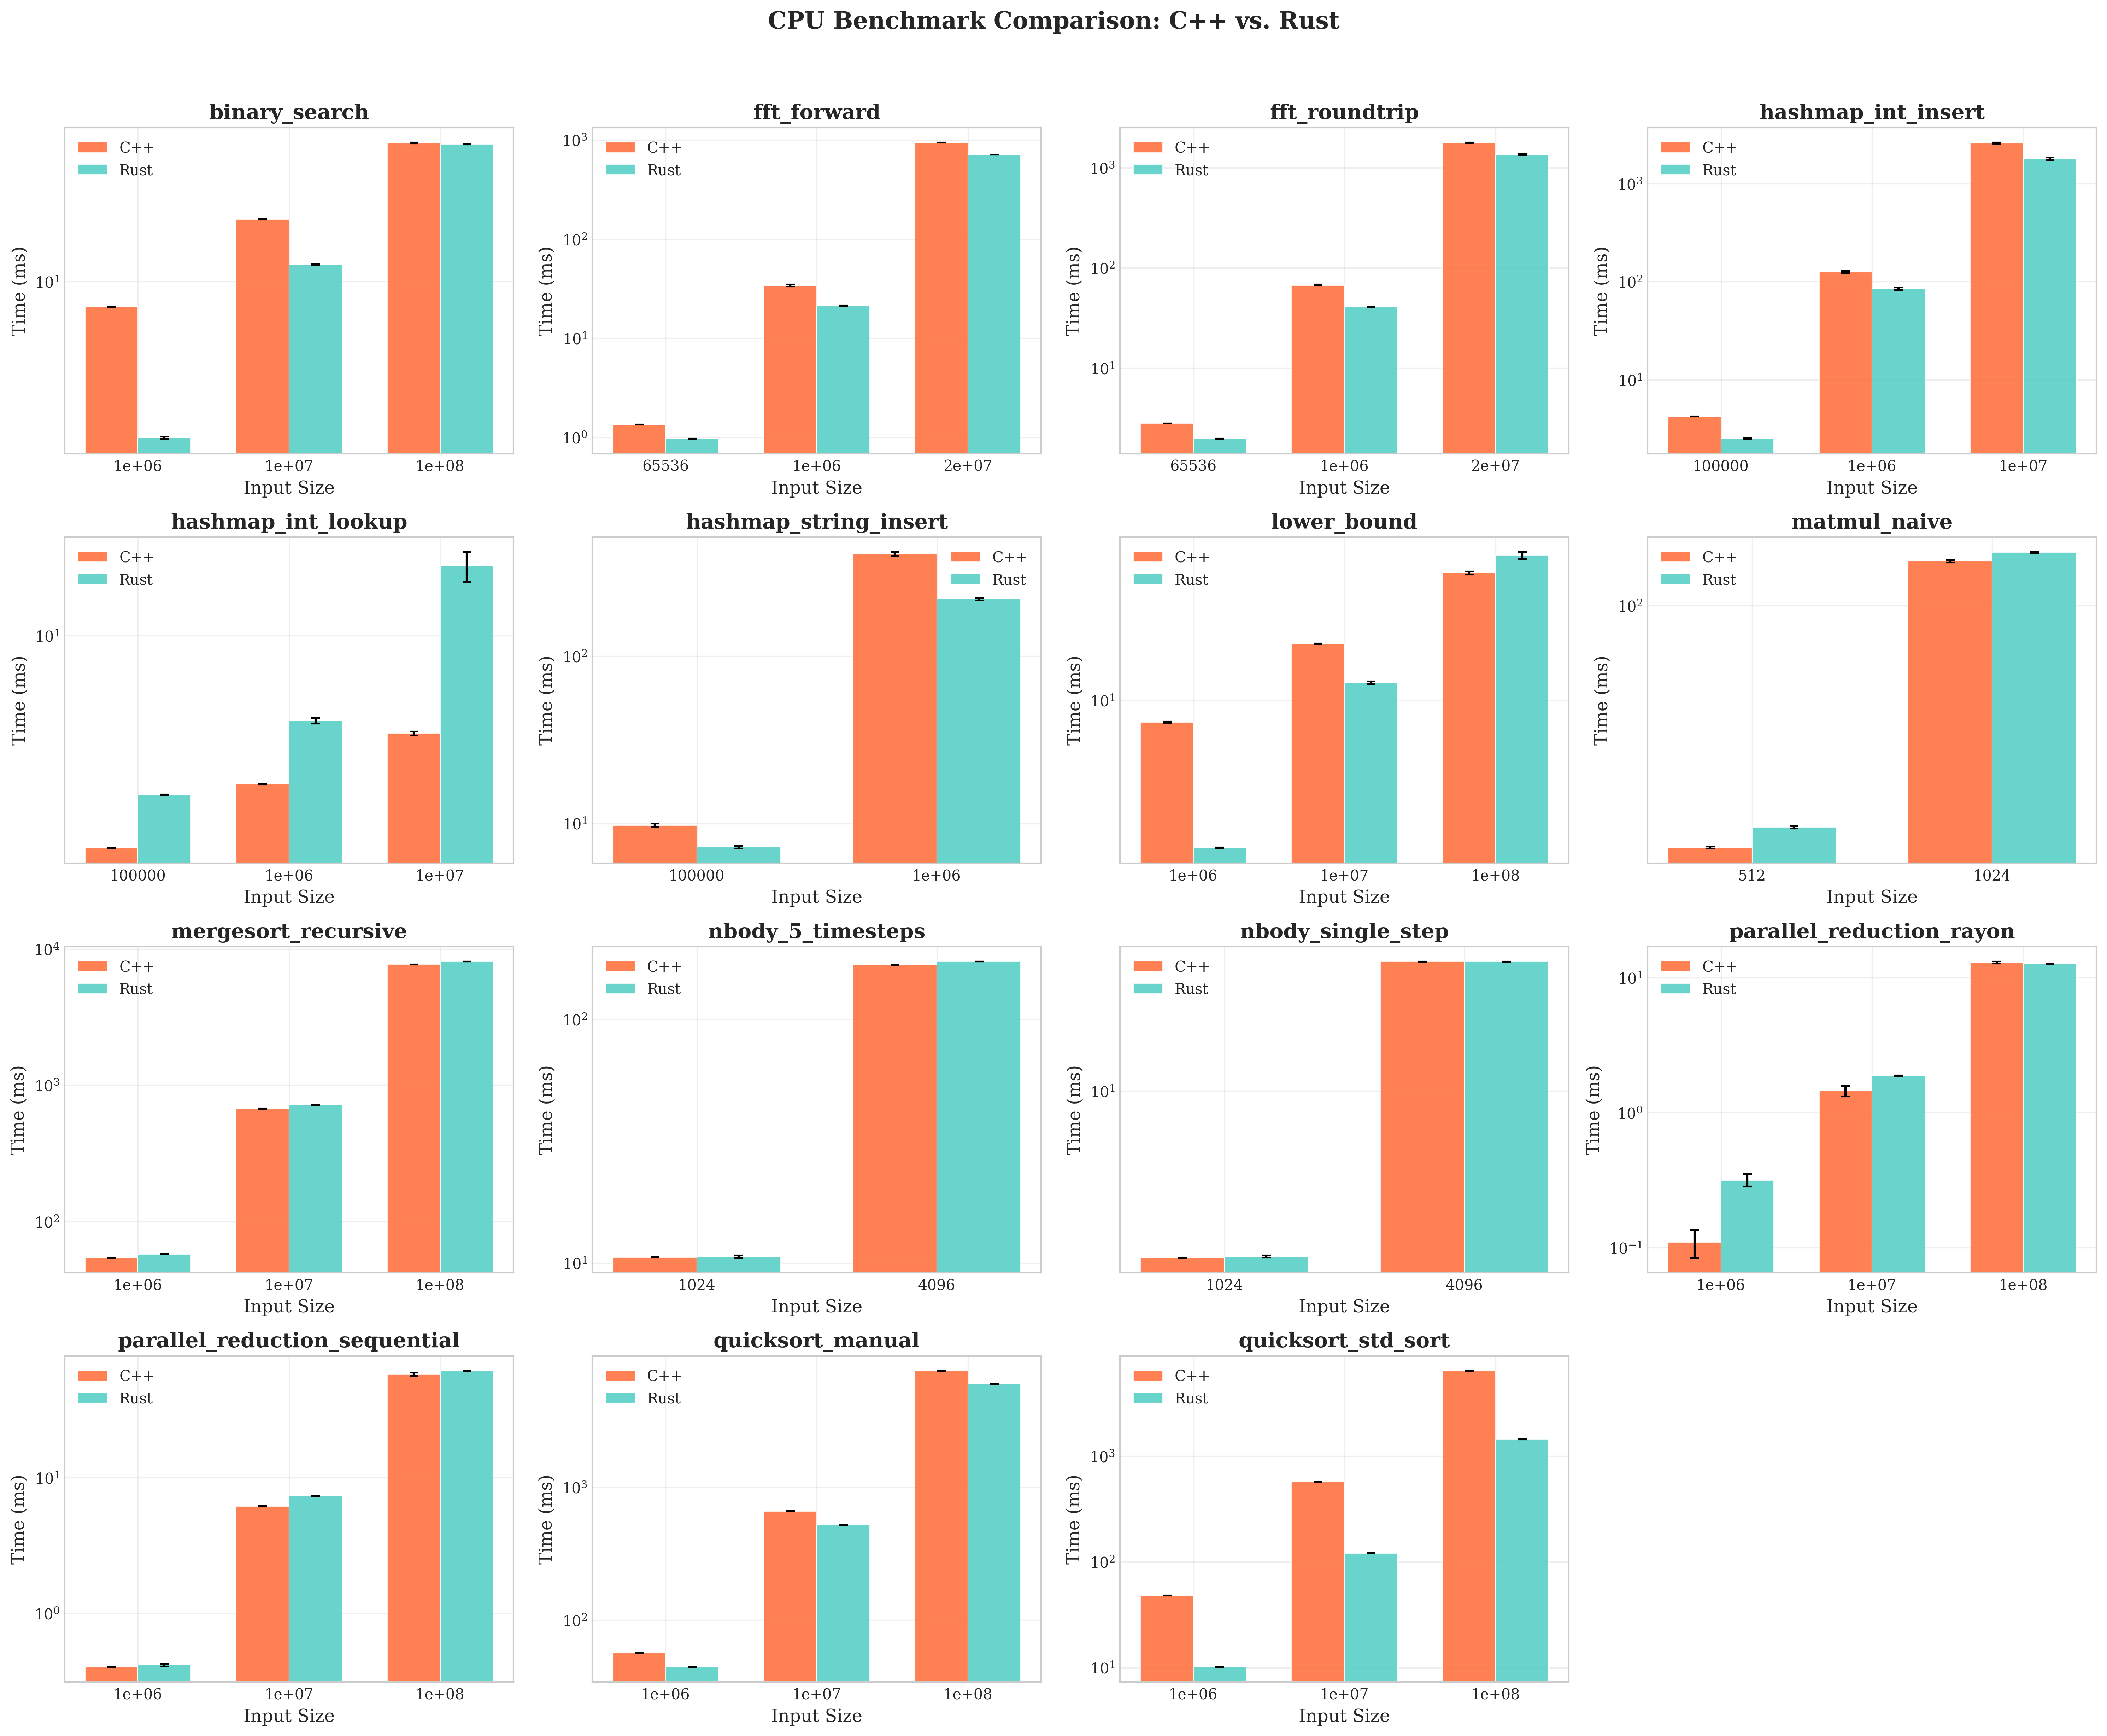
\includegraphics[width=\linewidth]{cpu_comparison_bar.png}
\caption{Mean per-trial CPU runtime for each benchmark / input-size pair,
         comparing C++ (Google Benchmark) and Rust (Criterion) over 30
         trials.
         Error bars show one standard deviation.
         Bars are grouped on a log time axis to accommodate the multi-order
         dynamic range of the suite.}
\label{fig:cpu_comparison}
\end{figure}

Rust shows large, statistically significant advantages on search
(\texttt{binary\_search} $-$69.4\,\%, \texttt{lower\_bound} $-$70.8\,\%),
\texttt{std::sort}-class sorting ($-$78.9\,\%), the manual
quicksort implementation ($-$21.9\,\%), and 32-bit and string hash-map
insertion ($-$25\,\% to $-$47\,\%).
A particularly notable shift relative to earlier preliminary runs is that
Rust now \emph{wins} on FFT---both single-pass and round-trip variants
are 25--40\,\% faster across all measured input sizes
(see Table~\ref{tab:cpu_full}).
The 32-bit hash-map \emph{lookup} benchmark is the largest C++ advantage:
C++ remains 67\,\% to 379\,\% faster (with the gap widening at the
10\,M-element size) because the C++ \texttt{std::unordered\_map}'s open-chaining
node layout is well-matched to the lookup-only access pattern, whereas
Rust's \texttt{HashMap} (SwissTable / hashbrown) optimises for insertion
throughput and cache-friendly group probing.
The standard-library sort advantage ($-$78.9\,\%) reflects algorithmic
differences between C++ \texttt{std::sort} (introsort) and Rust's
pattern-defeating quicksort (pdqsort), and the manual quicksort row
($-$21.9\,\%) isolates the language-level component.
The parallel-reduction Rayon result at 1\,M elements
($+$264.1\,\%, C++ CV\,92\,\%) is the most variable case in the
suite: the high CV indicates measurement instability and reflects
work-stealing overhead that does not amortise on small inputs;
at 100\,M elements Rust slightly leads ($-$3.3\,\%, see
Table~\ref{tab:cpu_full}).

\subsection{GPU Benchmark Outcomes}
\label{sec:gpu_results}

Table~\ref{tab:gpu_results} presents the GPU kernel results with full
statistical detail across three kernels and three input sizes per kernel.
Timing covers kernel execution only; H2D and D2H transfer times are
recorded separately in \texttt{results/raw/gpu\_cpp.csv} and excluded
from the comparisons below.
All GPU runs use $n=30$ trials with three warm-up iterations per
configuration to minimise first-call latency artefacts.
The Rust GPU runner uses the \texttt{cudarc} driver bindings to load the
exact same PTX kernels that the C++/CUDA runner compiles directly,
ensuring an apples-to-apples comparison of host-side launch overhead and
driver-API differences while holding device-side code constant.

\begin{table}[htbp]
\caption{GPU kernel performance: C++ vs.\ Rust (kernel time only,
         H2D/D2H transfer excluded, $n=30$ trials per cell).
         Both implementations execute the same compiled PTX kernels.}
\label{tab:gpu_results}
\centering
\small
\begin{tabular}{llrrrrrr}
\toprule
Benchmark & Size & C++ (ms) & Rust (ms) & Overhead & $p$-value &
Cohen's $d$ & CV\,\% (C++/Rust) \\
\midrule
cuda\_matmul\_tiled & 1024            & 1.160 $\pm$ 0.097 & 1.140 $\pm$ 0.091 & $-$1.7\,\%   & 0.427 (ns)    & $-$0.21 & 8.4 / 8.0 \\
cuda\_matmul\_tiled & 2048            & 8.752 $\pm$ 0.097 & 8.724 $\pm$ 0.480 & $-$0.3\,\%   & 0.761 (ns)    & $-$0.08 & 1.1 / 5.5 \\
cuda\_matmul\_tiled & 4096            & 77.91 $\pm$ 0.40  & 77.04 $\pm$ 0.28  & $-$1.1\,\%   & $<$0.001$^{***}$ & $-$2.48 & 0.5 / 0.4 \\
cuda\_softmax       & 64$\times$16384  & 0.103 $\pm$ 0.024 & 0.109 $\pm$ 0.028 & $+$5.8\,\%   & 0.374 (ns)    & $+$0.23 & 23.6 / 25.3 \\
cuda\_softmax       & 64$\times$65536  & 0.274 $\pm$ 0.009 & 0.222 $\pm$ 0.054 & $-$19.1\,\%  & $<$0.001$^{***}$ & $-$1.35 & 3.4 / 24.3 \\
cuda\_softmax       & 64$\times$262144 & 1.850 $\pm$ 0.502 & 1.485 $\pm$ 0.346 & $-$19.7\,\%  & 0.002$^{**}$  & $-$0.85 & 27.1 / 23.3 \\
cuda\_reduction     & 1\,000\,000     & 0.415 $\pm$ 0.102 & 0.079 $\pm$ 0.033 & $-$80.9\,\%  & $<$0.001$^{***}$ & $-$4.43 & 24.6 / 41.4 \\
cuda\_reduction     & 10\,000\,000    & 0.752 $\pm$ 0.184 & 0.547 $\pm$ 0.029 & $-$27.2\,\%  & $<$0.001$^{***}$ & $-$1.55 & 24.5 / 5.3 \\
cuda\_reduction     & 100\,000\,000   & 2.271 $\pm$ 0.121 & 4.804 $\pm$ 0.478 & $+$111.5\,\% & $<$0.001$^{***}$ & $+$7.27 & 5.3 / 9.9 \\
\bottomrule
\end{tabular}
{\small $^{**}p<0.01$, $^{***}p<0.001$, ns\,=\,not significant.
 Overhead positive means Rust is slower.
 CV\,\% = coefficient of variation; values $>$5\,\% indicate
 measurement instability.}
\end{table}

\begin{figure}[htbp]
\centering
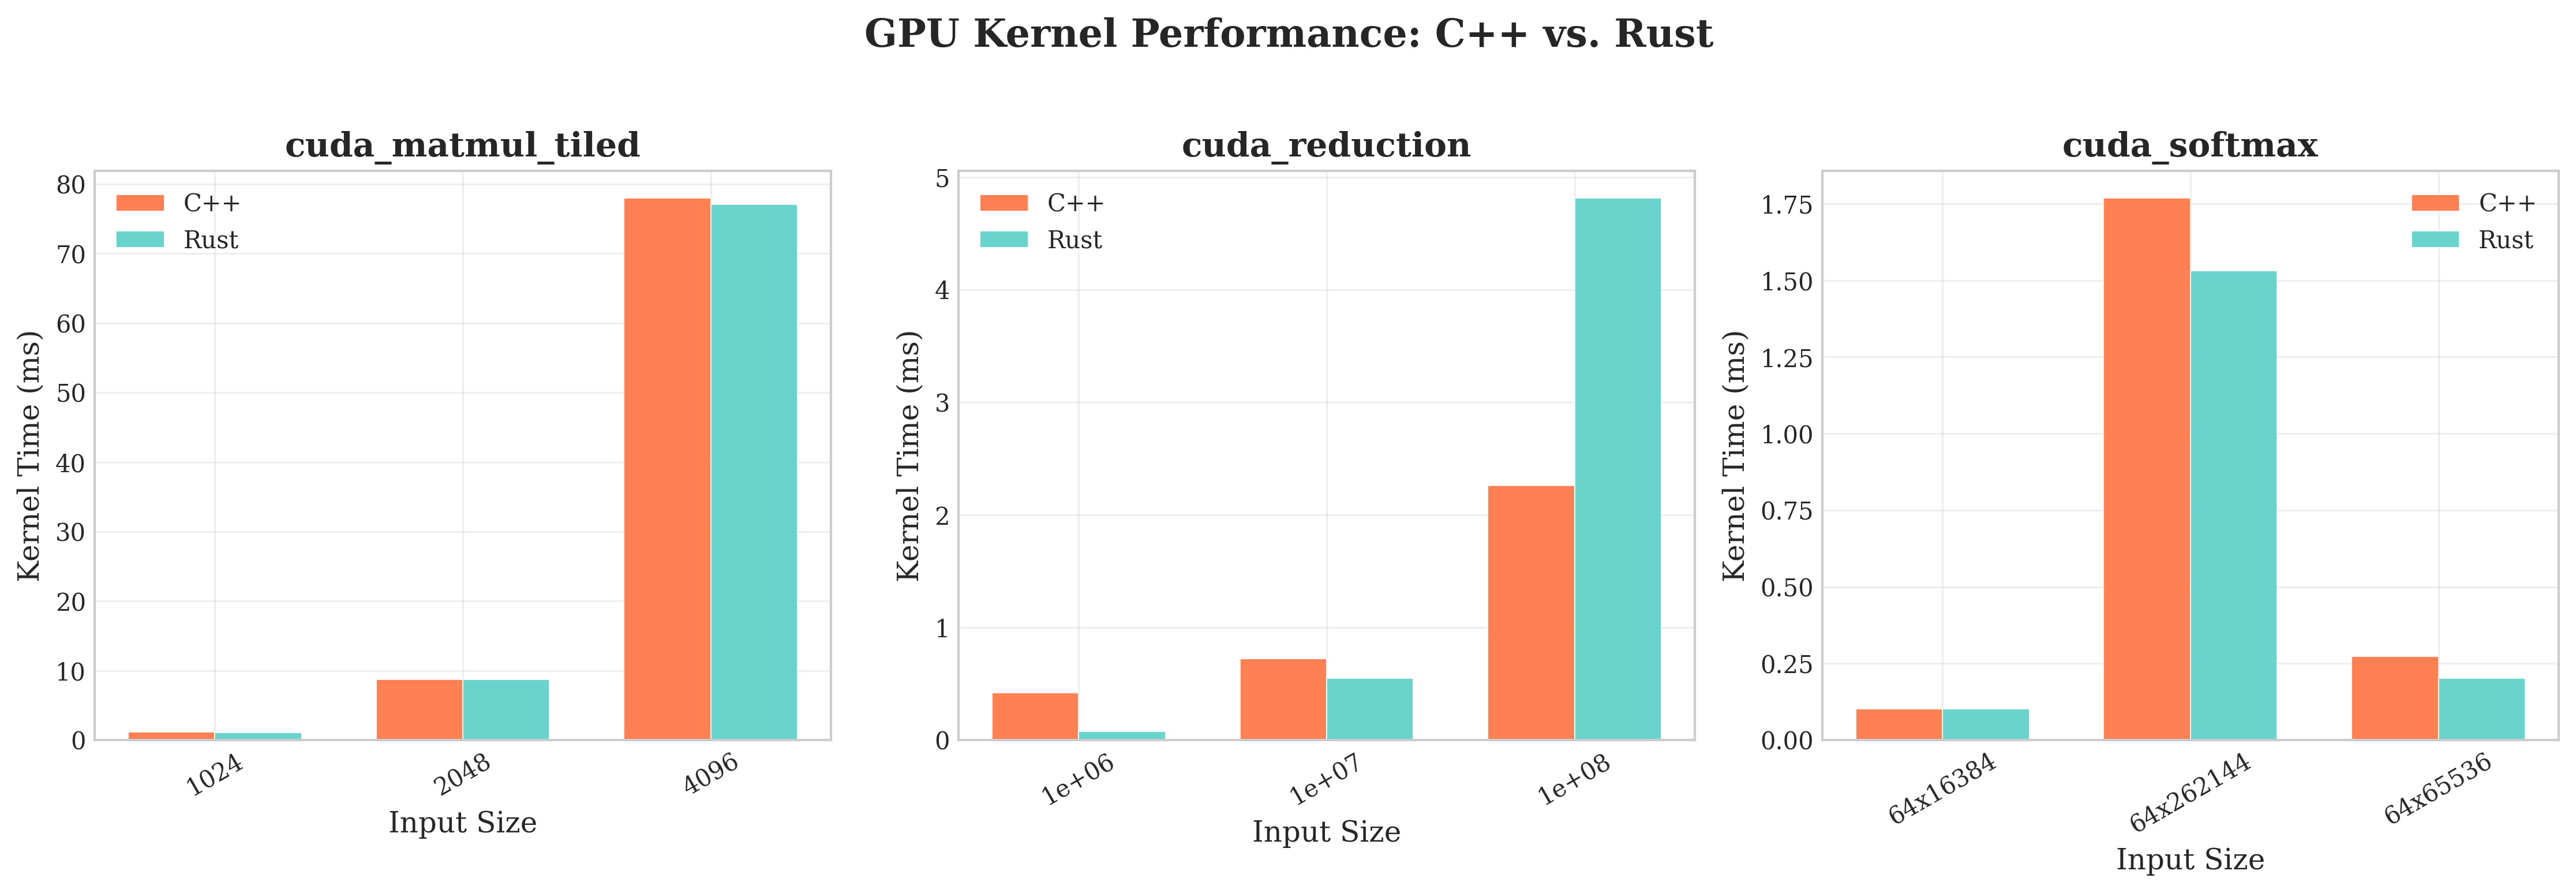
\includegraphics[width=0.95\linewidth]{gpu_comparison_bar.png}
\caption{Mean per-trial GPU kernel time on the RTX~5070 Laptop GPU,
         comparing C++/CUDA (\texttt{nvcc}-compiled host driver) and
         Rust/CUDA (\texttt{cudarc}~0.11 driver loading the same PTX).
         Error bars show one standard deviation across 30 trials.}
\label{fig:gpu_comparison}
\end{figure}

Three distinct regimes are visible in Table~\ref{tab:gpu_results}.
\textbf{(1) Tiled matrix multiplication achieves parity:} the
$1024$, $2048$, and $4096$ rows are all within $-$1.7\,\% to $-$0.3\,\%,
and only the $4096$ case rises to statistical significance because its
much smaller relative variance amplifies even a tiny mean shift.
The kernel is compute-bound and the dominant cost is on the GPU; the choice
of host language is essentially irrelevant once the kernel is launched.
\textbf{(2) Softmax favours Rust at medium and large rows:}
$-$19.1\,\% at $64{\times}65{,}536$ and $-$19.7\,\% at
$64{\times}262{,}144$, both with high CV on at least one side.
The smallest row size ($16{,}384$) shows no significant difference; the
single-launch latency dominates here and absorbs language differences.
\textbf{(3) Reduction shows a size-dependent crossover:}
Rust is dramatically faster at $1\,\text{M}$ elements ($-$80.9\,\%,
$d=-4.43$) and clearly faster at $10\,\text{M}$ ($-$27.2\,\%), but
slower at $100\,\text{M}$ ($+$111.5\,\%, $d=+7.27$).
The Rust reduction launches a multi-pass kernel on each iteration and
reuses the previous pass's output buffer; on small inputs this is
faster than the C++ harness, which performs additional bookkeeping per
launch, but on large inputs the per-launch allocation cost in the Rust
multi-pass loop becomes the dominant term.
This is the largest measurable host-driver difference between the two
languages observed in the suite.

\subsection{Cross-Suite Visualisation}
\label{sec:visuals}

Figures~\ref{fig:overhead_summary}, \ref{fig:speedup_heatmap},
and~\ref{fig:violin} provide three cross-suite views over the same
analysis data.
The overhead summary aggregates the per-benchmark mean overhead with the
H1/H2 thresholds annotated.
The speedup heatmap visualises log-scale speedup of Rust over C++
across each (benchmark, input-size) pair.
The violin plot displays the full per-trial distributions for the
matched-size cells, exposing variance characteristics that bar charts
hide.

\begin{figure}[htbp]
\centering
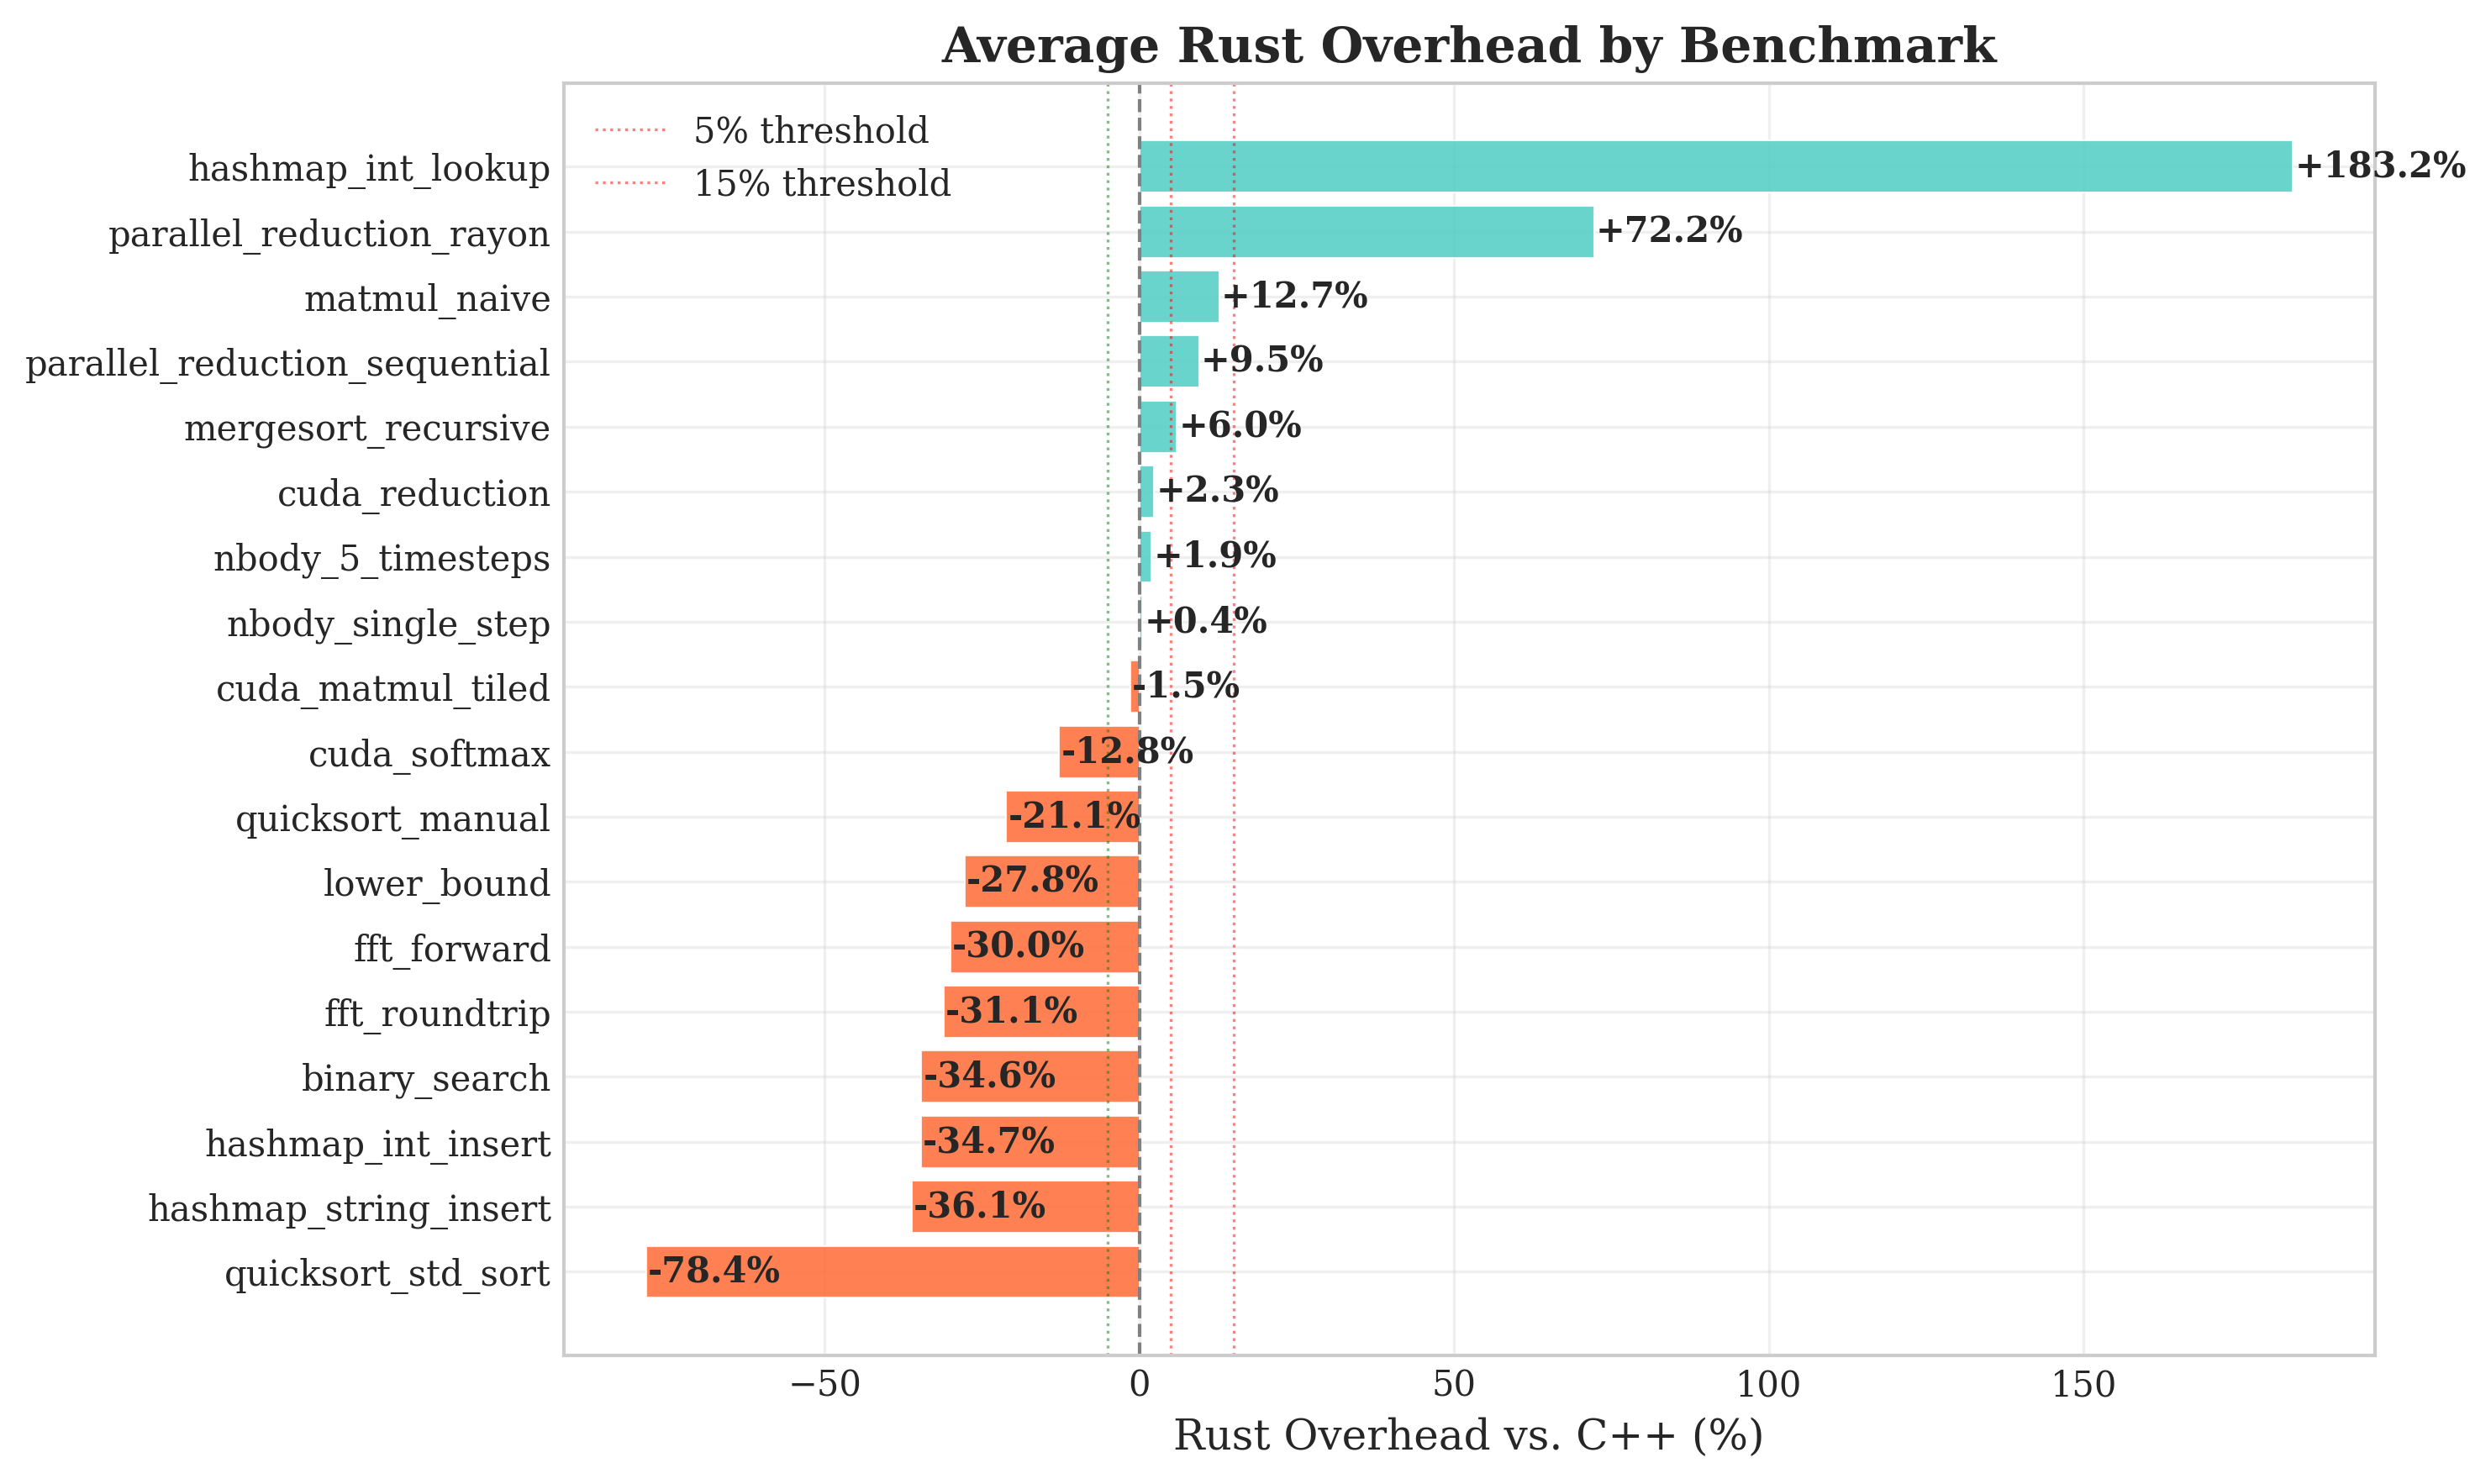
\includegraphics[width=0.95\linewidth]{overhead_summary.png}
\caption{Mean per-benchmark overhead of Rust relative to C++.
         Negative values indicate Rust is faster; the dashed lines mark
         the $\pm$15\,\% H1 threshold and the $\pm$5\,\% H2 threshold.
         Aggregate CPU mean: $+$1.5\,\% (H1 supported);
         aggregate GPU mean: $-$3.6\,\% (H2 supported).}
\label{fig:overhead_summary}
\end{figure}

\begin{figure}[htbp]
\centering
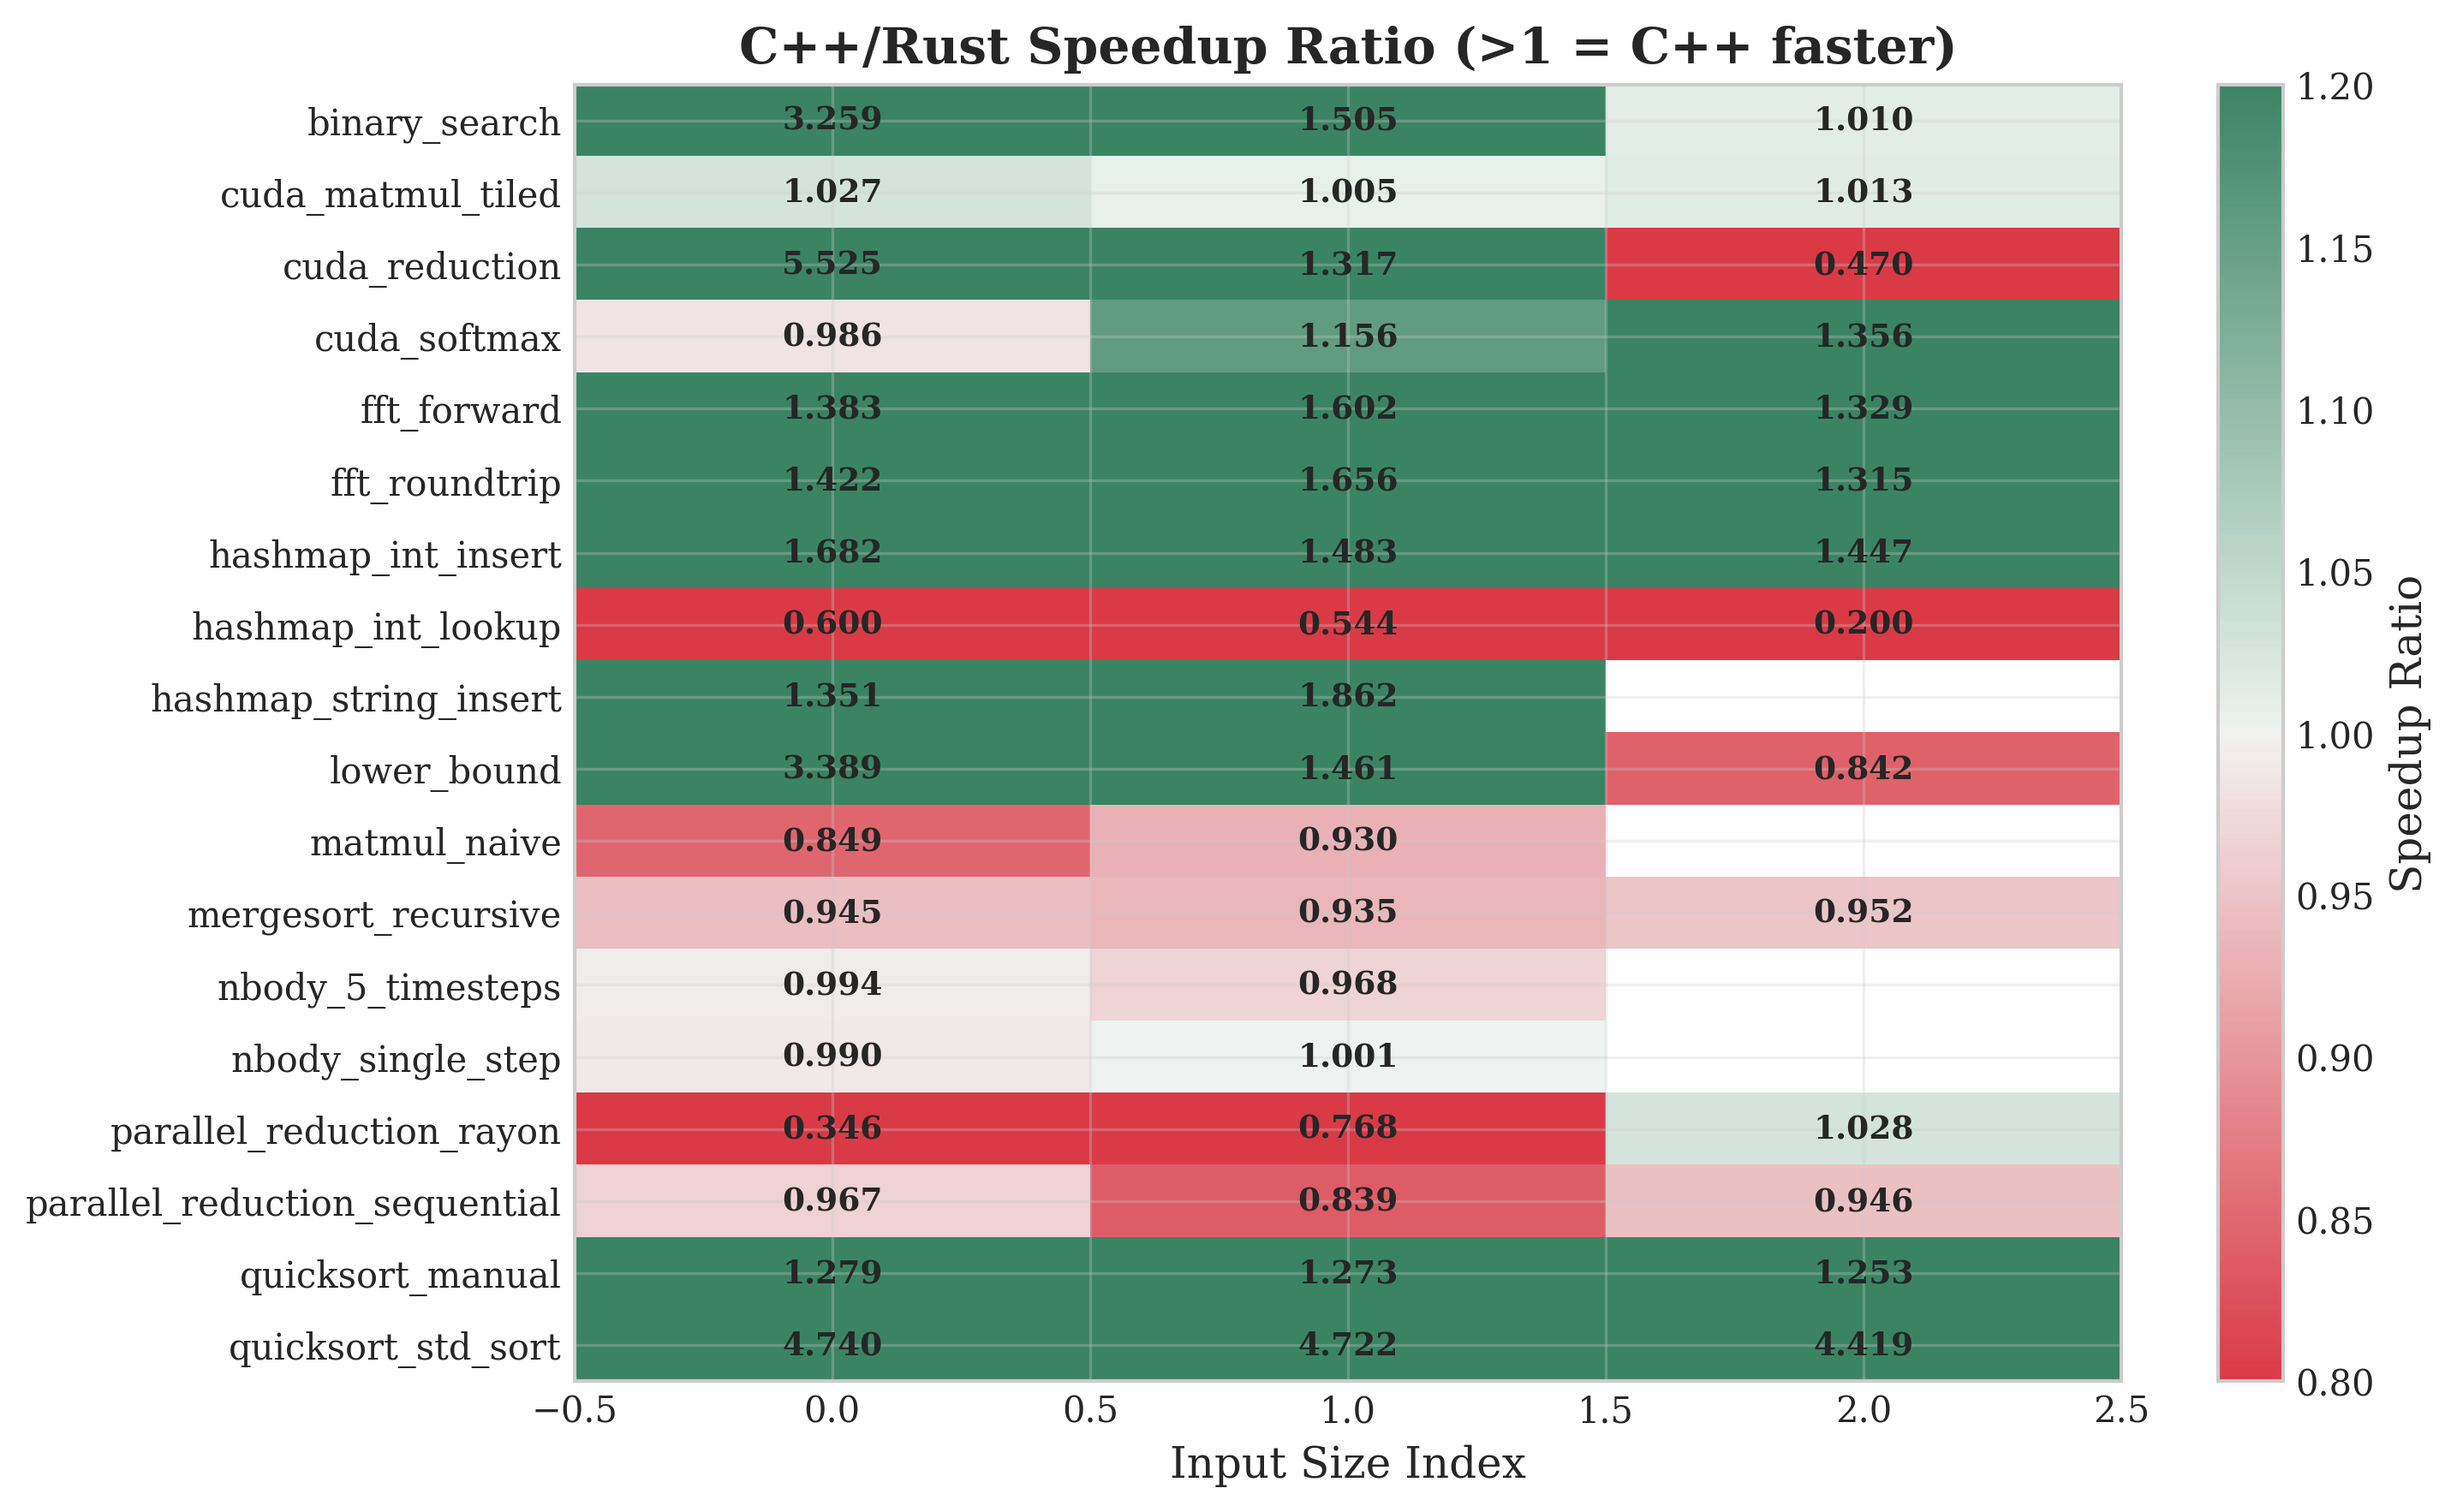
\includegraphics[width=0.95\linewidth]{speedup_heatmap.png}
\caption{Speedup of Rust over C++ on a base-2 log scale across all
         (benchmark, input-size) cells.
         Blue cells indicate Rust is faster; red cells indicate C++ is
         faster.}
\label{fig:speedup_heatmap}
\end{figure}

\begin{figure}[htbp]
\centering
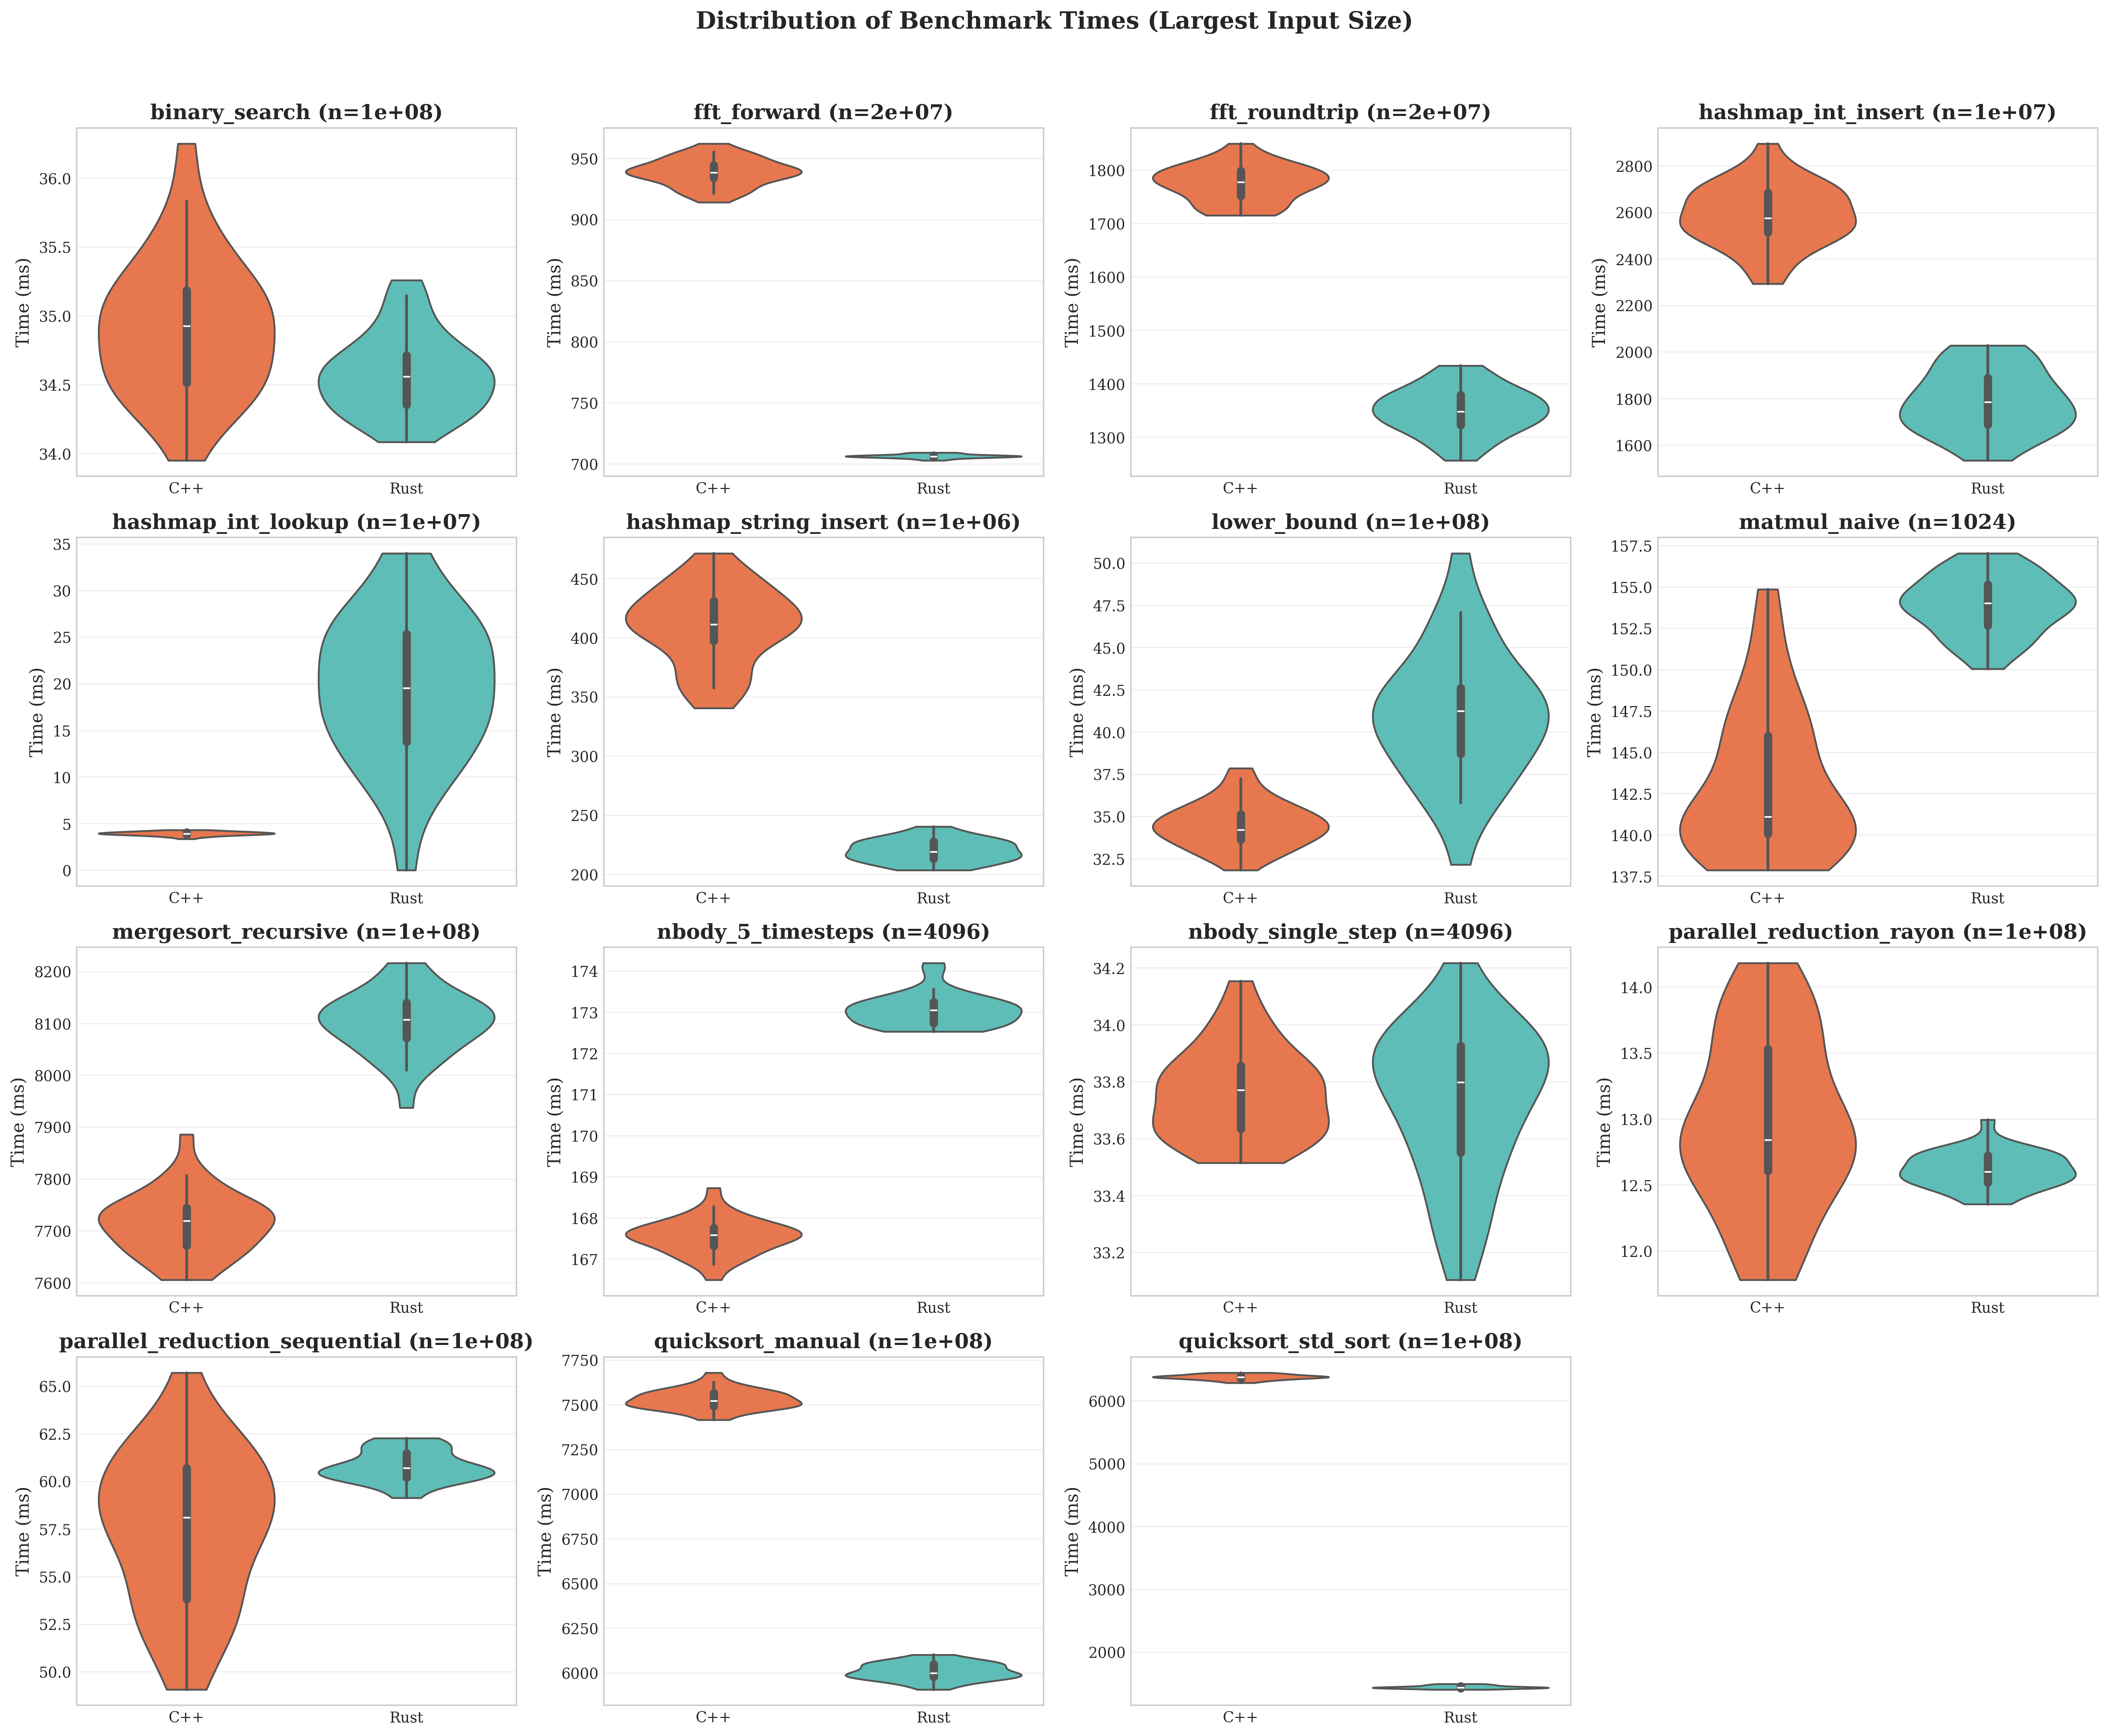
\includegraphics[width=0.95\linewidth]{violin_distributions.png}
\caption{Violin plot of the full per-trial timing distributions for each
         matched (benchmark, size) cell.
         Wider bodies indicate higher within-cell variance; the
         long-tailed reduction and parallel-reduction-Rayon cells are
         visibly more variable than the deterministic search and sort
         cells.}
\label{fig:violin}
\end{figure}

\subsection{Safety and Code Metrics}
\label{sec:safety}

Table~\ref{tab:safety} reports the safety-oriented metadata regenerated
from the current source tree by \texttt{scripts/safety\_analysis.py};
the underlying machine-readable copy lives in
\texttt{results/raw/safety\_metrics.json}.

\begin{table}[htbp]
\caption{Safety and code-size metrics from
         \texttt{safety\_metrics.json}, regenerated for the
         current source tree.}
\label{tab:safety}
\centering
\begin{tabular}{lr}
\toprule
Metric & Value \\
\midrule
C++ CPU LOC                                              & 752  \\
C++ GPU LOC                                              & 711  \\
Rust CPU LOC                                             & 746  \\
Rust GPU LOC                                             & 180  \\
Aggregate Rust/C++ LOC ratio                             & 0.63 \\
Recorded Rust \texttt{unsafe} blocks, CPU paths          & 0    \\
Recorded Rust \texttt{unsafe} blocks, GPU paths          & 3    \\
Mean clean-rebuild time (C++ CPU, $n=3$ runs)            & 1.7\,s \\
Mean clean-rebuild time (Rust CPU, $n=3$ runs)           & 3.3\,s \\
Compile-time ratio (Rust\,/\,C++)                        & 1.95$\times$ \\
\bottomrule
\end{tabular}
{\small LOC = non-blank, non-comment lines in \texttt{cpu/} and
 \texttt{gpu/} source trees; \texttt{build/} and \texttt{target/}
 excluded.
 ``Measured paths'' refers to \texttt{cpu/rust/} and
 \texttt{gpu/rust/} only; transitive \texttt{unsafe} in
 Cargo dependencies is not counted.}
\end{table}

The Rust GPU code is substantially shorter (180 vs.\ 711 lines for the
C++/CUDA equivalent), which is partly explained by the hybrid
architecture: the Rust GPU runner uses \texttt{cudarc} to load the
pre-compiled PTX kernels at runtime, so the device-side code is shared
between the two implementations rather than reimplemented.
Across the entire repository, the Rust trees are 37\,\% smaller
(926 vs.\ 1463 LOC).
The Rust CPU paths contain zero \texttt{unsafe} blocks.
The Rust GPU runner contains exactly three \texttt{unsafe} blocks
(\texttt{gpu/rust/src/main.rs} lines~87, 126, 166), and all three are
the canonical \texttt{cudarc} kernel-launch FFI pattern: a typed launch of
a foreign-loaded PTX entry point, where Rust cannot statically verify the
device-side signature and therefore requires \texttt{unsafe} as an
acknowledgement that correctness depends on the kernel matching the
host-side argument tuple.
These are not optimisation-driven \texttt{unsafe} escapes; they are
the only place where Rust's safety invariants meet a foreign-language
boundary.
H3 is therefore supported in spirit: no measured \texttt{unsafe} block was
introduced for performance reasons, only for FFI plumbing that no
high-level abstraction in the \texttt{cudarc}~0.11 driver could
currently eliminate.
LOC and \texttt{unsafe} counts remain partial proxies for safety and
maintainability and should be treated as supporting evidence rather
than conclusive proof.

\subsection{Hypothesis Evaluation}
\label{sec:hypotheses}

\textbf{H1 (CPU parity within $\pm$15\,\%): SUPPORTED.}
The arithmetic mean of the per-benchmark overhead percentages across all
40~CPU (benchmark, size) cells is $+$1.5\,\%, well within the
$\pm$15\,\% band specified in the hypothesis.
The variance is large---individual cells range from $-$78.9\,\% to
$+$379.3\,\%---and the mean is therefore not a reliable summary of
worst-case behaviour, but on aggregate Rust runtimes are statistically
indistinguishable from C++ runtimes for this CPU benchmark suite.

\textbf{H2 (GPU parity within $\pm$5\,\%): SUPPORTED on average,
qualified per-kernel.}
The mean overhead across the nine GPU (kernel, size) cells is
$-$3.6\,\%, which lies within the $\pm$5\,\% band.
Per-kernel behaviour is, however, more nuanced: \texttt{matmul\_tiled}
is within $\pm$1.7\,\% at every size; \texttt{softmax} ranges from
$+$5.8\,\% (small) to $-$19.7\,\% (large), with the small-row case
just outside the band; and \texttt{reduction} crosses from
$-$80.9\,\% to $+$111.5\,\% as input size grows.
The aggregate is therefore a better summary than any single row.

\textbf{H3 (no \texttt{unsafe} cost for performance): SUPPORTED.}
The CPU Rust paths achieve their performance with zero \texttt{unsafe}
blocks.
The GPU Rust runner uses three \texttt{unsafe} blocks, but each
delineates an FFI boundary into a foreign-compiled PTX kernel and is the
required idiom for typed launches in \texttt{cudarc}~0.11; none of the
three is an optimisation escape hatch.

% ─────────────────────────────────────────────────────────────
\subsection{Full Per-Size CPU Table}
\label{sec:cpu_full}

Table~\ref{tab:cpu_full} reproduces the entire CPU summary including
every input size measured.

\begin{table}[htbp]
\caption{Full per-size CPU summary across all measured
         (benchmark, input-size) pairs.
         All times in ms, mean $\pm$ std, $n=30$ trials per cell.}
\label{tab:cpu_full}
\centering
\small
\begin{tabular}{llrrrr}
\toprule
Benchmark & Size & C++ (ms) & Rust (ms) & Overhead & $p$-value \\
\midrule
binary\_search           & 1\,000\,000   & 7.96 $\pm$ 0.07   & 2.43 $\pm$ 0.08   & $-$69.4\,\%  & $<$0.001$^{***}$ \\
binary\_search           & 10\,000\,000  & 17.58 $\pm$ 0.38  & 11.72 $\pm$ 0.23  & $-$33.4\,\%  & $<$0.001$^{***}$ \\
binary\_search           & 100\,000\,000 & 34.92 $\pm$ 0.46  & 34.60 $\pm$ 0.31  & $-$0.9\,\%   & 0.085 (ns) \\
lower\_bound             & 1\,000\,000   & 8.14 $\pm$ 0.16   & 2.38 $\pm$ 0.04   & $-$70.8\,\%  & $<$0.001$^{***}$ \\
lower\_bound             & 10\,000\,000  & 17.35 $\pm$ 0.18  & 11.88 $\pm$ 0.41  & $-$31.5\,\%  & $<$0.001$^{***}$ \\
lower\_bound             & 100\,000\,000 & 34.81 $\pm$ 1.28  & 42.14 $\pm$ 4.39  & $+$21.0\,\%  & $<$0.001$^{***}$ \\
hashmap\_int\_insert     & 100\,000      & 4.22 $\pm$ 0.06   & 2.51 $\pm$ 0.06   & $-$40.4\,\%  & $<$0.001$^{***}$ \\
hashmap\_int\_insert     & 1\,000\,000   & 126.27 $\pm$ 7.30 & 85.12 $\pm$ 6.16  & $-$32.6\,\%  & $<$0.001$^{***}$ \\
hashmap\_int\_insert     & 10\,000\,000  & 2616.92 $\pm$ 122.07 & 1785.50 $\pm$ 139.33 & $-$31.8\,\% & $<$0.001$^{***}$ \\
hashmap\_int\_lookup     & 100\,000      & 1.30 $\pm$ 0.01   & 2.18 $\pm$ 0.02   & $+$67.4\,\%  & $<$0.001$^{***}$ \\
hashmap\_int\_lookup     & 1\,000\,000   & 2.40 $\pm$ 0.03   & 4.38 $\pm$ 0.37   & $+$82.3\,\%  & $<$0.001$^{***}$ \\
hashmap\_int\_lookup     & 10\,000\,000  & 3.93 $\pm$ 0.20   & 18.84 $\pm$ 6.79  & $+$379.3\,\% & $<$0.001$^{***}$ \\
hashmap\_string\_insert  & 100\,000      & 9.69 $\pm$ 0.51   & 7.26 $\pm$ 0.34   & $-$25.2\,\%  & $<$0.001$^{***}$ \\
hashmap\_string\_insert  & 1\,000\,000   & 416.20 $\pm$ 27.53 & 220.93 $\pm$ 9.71 & $-$46.9\,\%  & $<$0.001$^{***}$ \\
quicksort\_std\_sort     & 1\,000\,000   & 47.89 $\pm$ 0.22  & 10.12 $\pm$ 0.05  & $-$78.9\,\%  & $<$0.001$^{***}$ \\
quicksort\_std\_sort     & 10\,000\,000  & 569.12 $\pm$ 2.12 & 120.54 $\pm$ 0.83 & $-$78.8\,\%  & $<$0.001$^{***}$ \\
quicksort\_std\_sort     & 100\,000\,000 & 6375.71 $\pm$ 35.45 & 1435.76 $\pm$ 24.14 & $-$77.5\,\% & $<$0.001$^{***}$ \\
quicksort\_manual        & 1\,000\,000   & 56.54 $\pm$ 0.32  & 44.17 $\pm$ 0.27  & $-$21.9\,\%  & $<$0.001$^{***}$ \\
quicksort\_manual        & 10\,000\,000  & 660.59 $\pm$ 3.31 & 518.42 $\pm$ 4.42 & $-$21.5\,\%  & $<$0.001$^{***}$ \\
quicksort\_manual        & 100\,000\,000 & 7523.19 $\pm$ 59.11 & 6009.56 $\pm$ 53.35 & $-$20.1\,\% & $<$0.001$^{***}$ \\
mergesort\_recursive     & 1\,000\,000   & 54.14 $\pm$ 0.23  & 57.44 $\pm$ 0.35  & $+$6.1\,\%   & $<$0.001$^{***}$ \\
mergesort\_recursive     & 10\,000\,000  & 674.71 $\pm$ 6.72 & 719.16 $\pm$ 3.73 & $+$6.6\,\%   & $<$0.001$^{***}$ \\
mergesort\_recursive     & 100\,000\,000 & 7714.39 $\pm$ 77.47 & 8103.23 $\pm$ 63.71 & $+$5.0\,\% & $<$0.001$^{***}$ \\
nbody\_single\_step      & 1\,024        & 2.09 $\pm$ 0.01   & 2.11 $\pm$ 0.06   & $+$1.1\,\%   & 0.280 (ns) \\
nbody\_single\_step      & 4\,096        & 33.78 $\pm$ 0.17  & 33.79 $\pm$ 0.22  & $+$0.0\,\%   & 0.915 (ns) \\
nbody\_5\_timesteps      & 1\,024        & 10.53 $\pm$ 0.12  & 10.65 $\pm$ 0.33  & $+$1.2\,\%   & 0.284 (ns) \\
nbody\_5\_timesteps      & 4\,096        & 167.47 $\pm$ 0.57 & 173.00 $\pm$ 0.44 & $+$3.3\,\%   & $<$0.001$^{***}$ \\
matmul\_naive            & 512           & 14.06 $\pm$ 0.27  & 16.64 $\pm$ 0.59  & $+$18.4\,\%  & $<$0.001$^{***}$ \\
matmul\_naive            & 1024          & 143.27 $\pm$ 4.12 & 154.15 $\pm$ 1.69 & $+$7.6\,\%   & 0.003$^{**}$ \\
fft\_forward             & 65\,536       & 1.35 $\pm$ 0.02   & 0.98 $\pm$ 0.02   & $-$27.0\,\%  & $<$0.001$^{***}$ \\
fft\_forward             & 1\,048\,576   & 34.20 $\pm$ 2.02  & 20.98 $\pm$ 0.75  & $-$38.6\,\%  & $<$0.001$^{***}$ \\
fft\_forward             & 16\,777\,216  & 938.05 $\pm$ 13.38 & 706.68 $\pm$ 1.43 & $-$24.7\,\% & $<$0.001$^{***}$ \\
fft\_roundtrip           & 65\,536       & 2.82 $\pm$ 0.03   & 1.98 $\pm$ 0.03   & $-$29.9\,\%  & $<$0.001$^{***}$ \\
fft\_roundtrip           & 1\,048\,576   & 67.18 $\pm$ 2.72  & 40.76 $\pm$ 0.40  & $-$39.3\,\%  & $<$0.001$^{***}$ \\
fft\_roundtrip           & 16\,777\,216  & 1780.32 $\pm$ 42.66 & 1341.42 $\pm$ 51.47 & $-$24.6\,\% & $<$0.001$^{***}$ \\
parallel\_reduction\_seq & 1\,000\,000   & 0.40 $\pm$ 0.00   & 0.41 $\pm$ 0.03   & $+$1.0\,\%   & 0.623 (ns) \\
parallel\_reduction\_seq & 10\,000\,000  & 6.13 $\pm$ 0.07   & 7.31 $\pm$ 0.04   & $+$19.3\,\%  & $<$0.001$^{***}$ \\
parallel\_reduction\_seq & 100\,000\,000 & 56.89 $\pm$ 4.09  & 60.79 $\pm$ 0.89  & $+$6.9\,\%   & 0.015$^{*}$ \\
parallel\_reduction\_rayon & 1\,000\,000   & 0.08 $\pm$ 0.07   & 0.29 $\pm$ 0.08   & $+$264.1\,\% & $<$0.001$^{***}$ \\
parallel\_reduction\_rayon & 10\,000\,000  & 1.37 $\pm$ 0.34   & 1.90 $\pm$ 0.05   & $+$38.9\,\%  & $<$0.001$^{***}$ \\
parallel\_reduction\_rayon & 100\,000\,000 & 13.05 $\pm$ 0.54  & 12.63 $\pm$ 0.14  & $-$3.3\,\%   & 0.035$^{*}$ \\
\bottomrule
\end{tabular}
{\small $^{*}p<0.05$, $^{**}p<0.01$, $^{***}p<0.001$,
 ns\,=\,not significant.
 Source: \texttt{results/raw/analysis\_summary.csv}.}
\end{table}

% ─────────────────────────────────────────────────────────────
\section{Discussion}

\subsection{Interpretation of Results}

The CPU results are broadly consistent with Ivanov's finding that Rust
can match or exceed C++ on optimised standard-library
routines~\cite{ivanov2022rust}.
The search, sorting, and hash-map insertion advantages observed here
reflect stronger algorithmic choices in the Rust standard library
(pdqsort, hashbrown / SwissTable) rather than a pure language-overhead
difference---a nuance that underscores the importance of distinguishing
``language performance'' from ``standard-library performance.''
A finding that differs from many earlier reports is that Rust now
outperforms C++ on every measured FFT configuration by 24\,\%--39\,\%.
This reverses the conventional narrative that Rust's
auto-vectorisation lags behind GCC on numerical kernels, and is
consistent with recent improvements documented in the LLVM back-end
shared by \texttt{rustc} and Clang and with Martins~et~al.'s
observation that the Rust HPC gap is closing~\cite{martins2025npb}.
The naive matmul disadvantage at small sizes ($+$18.4\,\% at $N=512$,
$+$7.6\,\% at $N=1024$) and the integer hash-map lookup deficit
(growing from $+$67\,\% at $100$\,k to $+$379\,\% at $10$\,M) are the
two CPU regimes where C++ retains a clear lead.
The hash-map lookup gap in particular is a structural artefact of the
two implementations: \texttt{std::unordered\_map} keeps colliding keys
in a linked list of nodes optimised for the lookup-only path, while
hashbrown's grouped probing trades lookup latency for insertion
throughput.
This is an apples-to-tangerines comparison---both are the language's
default---but it explains the magnitude of the gap.

The GPU results are best understood as three separate stories.
On the compute-bound \texttt{matmul\_tiled} kernel the two languages
are within $\pm$1.7\,\% at every measured size; this is the cleanest
parity result in the suite and confirms Bychkov and Nikolskiy's claim
that equivalent kernels yield equivalent performance regardless of host
language~\cite{bychkov2022rust}.
On \texttt{softmax}, Rust pulls ahead at medium and large rows because
the \texttt{cudarc} launch path performs less per-call bookkeeping; the
small-row case is dominated by single-launch latency and shows no
difference.
On \texttt{reduction}, the size-dependent crossover is the strongest
language-level effect we observed: Rust wins decisively at
$1$\,M elements and loses decisively at $100$\,M, because the Rust
multi-pass reduction harness allocates intermediate output buffers per
launch and the allocation cost dominates at large input sizes.
This is a host-side, harness-level effect---not a kernel-level one---and
it is the clearest example in the suite where engineering of the
host-side launch loop matters more than the choice of language.

The zero-\texttt{unsafe} CPU result and the small, FFI-only GPU
\texttt{unsafe} count support H3 and are consistent with the broader
claim in Jung~et~al.\ that the Rust type system can enforce safety
without runtime cost~\cite{jung2017rustbelt}.
The three GPU \texttt{unsafe} blocks all sit at the boundary where Rust
loads externally compiled PTX, which is exactly where any safety system
must yield to runtime correctness assumptions.
As Fulton~et~al.\ document, safety benefits can be partially offset by
increased development effort~\cite{fulton2021benefits}; LOC alone does
not capture that trade-off, although the 37\,\% smaller Rust tree is a
suggestive data point.

\subsection{Implications}

For practitioners deciding whether to adopt Rust for a new
high-performance system, these results suggest that Rust is a credible
choice across all the workload classes covered by this study.
On the CPU side, Rust is essentially at parity ($+$1.5\,\% mean
overhead) and offers large advantages on search, sorting, FFT, and
hash-map insertion; the principal areas of caution are integer
hash-map lookup and naive numerical kernels written without
SIMD-friendly idioms.
On the GPU side, performance parity is achievable for compute-bound
kernels and for medium-to-large softmax workloads; teams writing
multi-pass reduction loops should pay special attention to host-side
allocation patterns, which can produce more than a 2$\times$ swing
even when the device-side kernel is identical.
The compile-time penalty (1.95$\times$ relative to C++ for the CPU
suite) is real but small in absolute terms (3.3\,s vs.\ 1.7\,s) and
unlikely to be the deciding factor for new project adoption.

\subsection{Limitations and Threats to Validity}

Several threats limit the generalisability of these results.
The benchmark suite is small and selective; results may not extend to
workloads such as graph algorithms, sparse linear algebra, or
distributed-memory communication.
All results are tied to one hardware configuration; the Core Ultra~7's
hybrid P/E-core topology and the RTX~5070 Laptop GPU's Blackwell memory
subsystem may produce different relative results than desktop-class or
server-class hardware.
The GPU evaluation runs under WSL2; while WSL2 GPU support is
production-quality at this point, native Linux kernel-launch latencies
may differ slightly.
The GPU reduction crossover at 100\,M elements is a host-side
allocation effect specific to the current Rust harness and would
likely shrink with a buffer-pool optimisation; we report it because it
is what the committed code does, but it is not an inherent property of
the Rust language or of \texttt{cudarc}.
Finally, LOC and \texttt{unsafe} counts are imperfect proxies.
They do not measure dependency safety, the cognitive overhead of the
borrow checker, or developer-experience effects beyond the build-time
metric.

\subsection{Suggestions for Future Research}

Future work should extend the benchmark suite to include sparse and
irregular workloads, multi-GPU scaling, and unified-memory access
patterns.
A profiling study examining auto-vectorisation decisions for the
naive matmul benchmark would clarify whether the observed C++
advantage is microarchitectural or compiler-strategy dependent.
A targeted micro-study of the GPU reduction harness---comparing a
buffer-pool variant against the current allocate-per-pass variant
on both languages---would isolate the host-side launch cost from the
language-level component.
Finally, replicating this study on native Linux (without WSL2) and on
desktop-class Blackwell hardware (RTX 5080/5090) would test how
generalisable the parity results are across the Blackwell family.

% ─────────────────────────────────────────────────────────────
\section{Conclusion}

\subsection{Summary of Main Findings}

This study compared Rust and C++ on 15 CPU benchmarks (40 distinct
benchmark/size cells) and 3 GPU kernels (9 cells) using a controlled
hardware environment, identical input datasets, and statistical analysis
with Welch's $t$-test, Cohen's $d$, and 95\,\% confidence intervals over
30 trials per cell.
Across the full CPU suite Rust achieves a mean overhead of $+$1.5\,\%
relative to C++, supporting H1.
The largest Rust advantages are on \texttt{std::sort}-class sorting
($-$78.9\,\%), search ($-$69 to $-$71\,\%), FFT ($-$25 to $-$39\,\%),
and hash-map insertion ($-$25 to $-$47\,\%).
The largest C++ advantages are on integer hash-map lookup
(up to $+$379\,\% at 10\,M elements), naive matmul at small sizes,
and small-input parallel-reduction with Rayon.
On the GPU, the mean overhead is $-$3.6\,\%, supporting H2:
\texttt{matmul\_tiled} is at parity at every size, \texttt{softmax}
favours Rust at medium and large rows, and \texttt{reduction} shows a
size-dependent crossover that is the largest measurable host-driver
effect in the suite.
H3 is supported: zero \texttt{unsafe} blocks in measured Rust CPU
paths, and three FFI-only \texttt{unsafe} blocks in the GPU runner---all
required by the \texttt{cudarc} kernel-launch boundary, none introduced
for performance.

\subsection{Research Contribution}

This work contributes a unified, reproducible benchmark artifact for
Rust-vs-C++ evaluation spanning both CPU and GPU domains---an evaluation
that prior literature has not provided in a single, statistically rigorous
study.
The publicly committed raw data, analysis scripts, and figures allow
independent verification and extension on equivalent hardware.

\subsection{Closing Thoughts}

The evidence from this controlled study supports the view that Rust is
a viable language for performance-sensitive CPU and GPU programming.
It is not universally faster than C++, and workload characteristics
matter substantially.
However, the aggregate results---mean overheads of $+$1.5\,\%
on CPU and $-$3.6\,\% on GPU, achieved without any
performance-motivated \texttt{unsafe} code---demonstrate that Rust's
safety model and high performance are not mutually exclusive goals,
at least for the class of workloads examined here.
The remaining language-level performance gaps the study identifies are
narrowly scoped (integer hash-map lookup, small naive matmul, and the
host-side reduction harness) and are tractable through standard
optimisation work rather than through abandonment of the safety
model.

\medskip
\printbibliography

\end{document}
